% LaTeX file for resume 
% This file uses the resume document class (res.cls)

\documentclass{article} 
% the margin option causes section titles to appear to the left of body text 
\textwidth=5.2in % increase textwidth to get smaller right margin
%\usepackage{helvetica} % uses helvetica postscript font (download helvetica.sty)
%\usepackage{newcent}   % uses new century schoolbook postscript font 
\usepackage{url}
\usepackage{hyperref}
\hypersetup{
  % colorlinks,
  final,
  pdftitle={Equivariant Dendroidal Segal Spaces},
  pdfauthor={Bonventre, P. and Pereira, L. A.},
  % pdfsubject={Your subject here},
  % pdfkeywords={keyword1, keyword2},
  linktoc=page
}

\usepackage{xr}
\externaldocument{EqSegSp&G-infty-ops}

\input{commands.tex}%

%-------- TIKZ -----------------------------------------
\usepackage{tikz}%
\usetikzlibrary{matrix,arrows,decorations.pathmorphing,
cd,patterns,calc}
\tikzset{%
  treenode/.style = {shape=rectangle, rounded corners,%
                     draw, align=center,%
                     top color=white, bottom color=blue!20},%
  root/.style     = {treenode, font=\Large, bottom color=red!30},%
  env/.style      = {treenode, font=\ttfamily\normalsize},%
  dummy/.style    = {circle,draw,inner sep=0pt,minimum size=2mm}%
}%

\usetikzlibrary[decorations.pathreplacing]
% \usetikzlibrary{external}\tikzexternalize
% \makeatletters
% \renewcommand{\todo}[2][]{\tikzexternaldisable\@todo[#1]{#2}\tikzexternalenable}

% \makeatother

\begin{document} 
 
\title{Edits to ``Equivariant dendroidal Segal spaces and $G$-$\infty$-operads'' (v.4)
\\[12pt]} % the \\[12pt] adds a blank line after name
 
\author{Bonventre, P. and Pereira, L. A.}
 
\maketitle
 
The referee's preliminary report had two main sections:
first, they highlighted two key points where unclear notation prevented further reading of those sections; % of great narrative difficulty,
and second, they offered a numbered list of recommendations and suggestions.
We have implemented the vast majority of the changes recommended by the referee, and modified the discussion at many points to minimize confusion and provide additional detail.
The updates are organized into four categories:
\begin{itemize}
\item in ``Requested Revisions'', we address the two key pieces of unclear notation.
\item in ``Comments and departures'', we answer questions posed by the referee, and indicate where and why we departed from the referee's suggestions.
\item in ``Changes'', we address suggestions which required more significant edits,
% to the article, or small changes regarding errors which had inhibited mathematical understanding. These changes have themselves been grouped thematically.
and which we group thematically.
\item in ``Minor changes and typos'', we list fixed typos and other small corrections. % made in response to errors which did not appear to affect the referee's understanding.
\end{itemize}

Our updates are numbered by the corresponding numbered item in the referee report,
and all internal references have been modified to match the new numbering from the updated article.



\section{Requested revisions}

% The two locations which caused the referee confusion have been been updated.

\begin{itemize}
\item The first location, at the beginning of \S 5.2, was an unfortunate typo: %, if a maximally confusing one:
      in \eqref{OTIMESOC_EQ}, $\otimes_{\Omega[C]}$ has been changed to $\coprod_{\Omega[C]}$.
      We have also added context by recalling a similar decomposition of the product of 1-simplexes.

\item
% The second concerned the category $K \ltimes \mathbb R$, found in the Appendix.
      We have clarified the definition of the category $K \ltimes \mathbb R$ in Notation \ref{KLTIMES NOT},
      providing an explicit description and motivation for the notation.
      %, a precise definition, and two examples.
\end{itemize}

      

\section{Comments and departures} % Departures from suggestions/direct answer to comments

\begin{itemize}
\item[4.] We are firmly convinced that the definitions of node, stump and root from \cite[Defs. 5.7 and 5.9]{Per18}
are correct as stated. For example, consider the tree
\begin{equation}\label{FIRSTTREE2 EQ}
	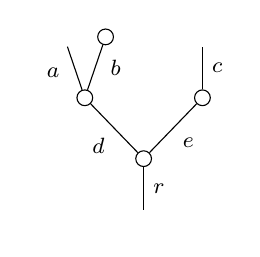
\begin{tikzpicture}[auto,grow=up,
	level distance = 2.2em,
	every node/.style={font=\footnotesize,minimum size=1.5mm}]%
	\tikzstyle{level 2}=[sibling distance=4.25em]%
	\tikzstyle{level 3}=[sibling distance=1.5em]%
		\node at (0,0)[font=\normalsize]{}%
			child{node [dummy] {}%
				child{node [dummy] {}%
					child{node {}%
					edge from parent node [swap] {$c$}}%
				edge from parent node [swap] {$e$}}%
				child{node [dummy] {}%
					child{node[dummy] {}%
					edge from parent node [very near end,swap] {$b$}}%
					child{node {}%
					edge from parent node [very near end] {$\phantom{b}a$}}%
				edge from parent node {$d$}}%
			edge from parent node [swap] {$r$}};%
	\end{tikzpicture}%
\end{equation}
The tuples $\underline{e}$ such that $\underline{e} < r$
are $de, dc, abe, abc, ae, ac$, and $r^{\uparrow} = de$ is the maximum of these (in the partial order on tuples $T^+$ as in \cite[Prop. 5.6]{Per18}). On a side note, that this maximum is unique reflects the statement that the generators of a free category/operad are characterized as the indecomposable operations (with symmetric action caveats in the operad case).

We are also unsure of how replacing ``maximum'' with ``upper bound'' would change the definitions, since an upper bound of a subset $A$ that is also in $A$ must be the maximum of $A$.  %

% To show that replacing "maximum" with "maximal" also is insufficient, consider the broad poset $X = \set{a,b_1,b_2}$ with (non-trivial) relations $b_1 \leq a$ and $b_2 \leq a$. Then $a$ is a root, $b_1$ and $b_2$ are leaves, but $a$ is not a node: the unary tuples $b_1$ and $b_2$ are incomparable maximal tuples above $a$.
    


\end{itemize}


{\color{red} HERE}

\section{Minor appendix changes}

\begin{itemize}

\item[2.] Fixed $\{\mathcal{F}_r\}$
to $\mathcal{F}_r$ in Lemma A.27(ii)
     
\item[3.] Replaced ``analogue'' with ``analogous'' in the proof of Lemma A.27(ii)

\item[4.]
In the last line of the proof of Lemma A.27(ii),
replaced ``(i) again...'' with ``Part (i) again...''
so as not to start sentence with ``(i)''.

{\color{red} HERE}



                           
\end{itemize}








\section{Minor changes and typos}
 
% The following lists the corrections of typos and other smaller mistakes listed in the preliminary referee report.

\begin{itemize}
	\item cat
\end{itemize}







\bibliography{biblio}{}

\bibliographystyle{alpha}


\end{document} 




%%% Local Variables:
%%% mode: latex
%%% TeX-master: t
%%% End:
